\section{组件}
\subsection{组件布局}
\indent\urwid{} 利用组件分割屏幕空间. 使得实现动态的界面十分容易, 可以适应不同的终端和字体大小. \cref{fig:example_of_widget_layout} 是一个 \urwid{} 布局的例子.

\begin{figure}[!htb]
    \centering
    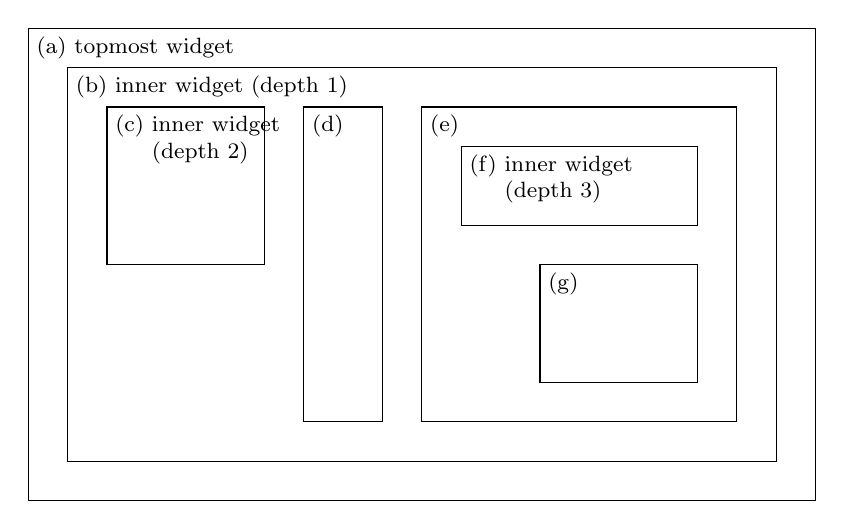
\begin{tikzpicture}[
  block/.style = {rectangle, draw},
  number/.style = {anchor = north west, inner sep = 3pt, font = \footnotesize, align = flush left}
]
  \node[block, minimum width = 10cm, minimum height = 6cm]   (a) at (5,   5.5)  {};
  \node[block, minimum width = 9cm,  minimum height = 5cm]   (b) at (5,   5.5)  {};
  \node[block, minimum width = 2cm,  minimum height = 2cm]   (c) at (2,   6.5)  {};
  \node[block, minimum width = 1cm,  minimum height = 4cm]   (d) at (4,   5.5)  {};
  \node[block, minimum width = 4cm,  minimum height = 4cm]   (e) at (7,   5.5)  {};
  \node[block, minimum width = 3cm,  minimum height = 1cm]   (f) at (7,   6.5)  {};
  \node[block, minimum width = 2cm,  minimum height = 1.5cm] (g) at (7.5, 4.75) {};
  
  \node[number] at (a.north west) {(a) topmost widget};
  \node[number] at (b.north west) {(b) inner widget (depth 1)};
  \node[number] at (c.north west) {(c) inner widget\\\hphantom{(c) }(depth 2)};
  \node[number] at (d.north west) {(d)};
  \node[number] at (e.north west) {(e)};
  \node[number] at (f.north west) {(f) inner widget\\\hphantom{(f) }(depth 3)};
  \node[number] at (g.north west) {(g)};
\end{tikzpicture}
    \caption{\urwid{} 布局举例}
    \label{fig:example_of_widget_layout}
\end{figure}